\scanpage{203}
% archive sheet number: 202

\figure{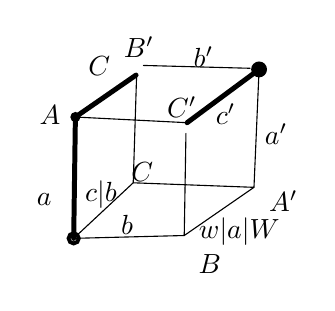
\begin{tikzpicture}[scale=.72,line cap=round]
\draw (0,0)--(1.95,.05)--(3.18,.90)--(3.27,2.98)--(2.0,2.04)--(.03,2.14)--(1.11,2.88) (1.23,3.05)--(3.11,3.00) (1.05,.98)--(1.11,2.88) (0,0)--(1.05,.98)--(3.18,.90) (1.95,.05)--(1.98,1.85);
\draw[line width=1.8pt] (0,0)--(.03,2.14)--(1.1,2.88) (2.0,2.04)--(3.27,2.98);
\fill (.03,2.14) circle (.09) (3.27,2.98) circle (.14);
\draw[line width=1.4pt] (0,0) circle (.09);
\node at (.45,3.04) {$\deleted{\unsure{C}}$};\node at (1.15,3.37) {$B'$};\node at (2.29,3.2) {$b'$};
\node at (-.42,2.18) {$A$};\node at (1.91,2.31) {$C'$};\node at (2.68,2.19) {$c'$};
\node at (3.57,1.84) {$a'$};\node at (-.52,.68) {$a$};\node at (.48,.78) {$\unsure{c|b}$};
\node at (1.21,1.17) {$C$};\node at (.94,.24) {$b$};\node at (2.40,-.45) {$B$};
\node at (2.92,.12) {$\unsure{w|a|W}$};\node at (3.70,.66) {$A'$};
\end{tikzpicture}}

% slanted
\margin{\tikz[baseline=(s.base)]\node[draw,ellipse,rotate=9,inner sep=4pt] (s) {Trop lourd};}

\[
 \begin{aligned}
 &\Sigma_{a\unsure{\prime}}\quad\Sigma_b\quad\Sigma_c\quad\Sigma_{AB'}\quad{}^{\unsure{-}}\Sigma_{BC'}\quad\Sigma_{CB'}\quad\Sigma_{CA'}\quad\Sigma_{AC'}\\
 &\Sigma_{a'}\quad\Sigma_{b'}\quad\Sigma_{c'}
 \end{aligned}
\]

\[
 \left\{\begin{aligned}
 \Sigma_a+\Sigma_{c'}&=\Sigma_{AB'}+\Sigma_{BC'}\\
 \Sigma_a+\Sigma_{b'}&=\Sigma_{AC'}+\Sigma_{CB'}\\
 \Sigma_b+\Sigma_{a'}&=\Sigma_{BC'}+\Sigma_{CA'}\\
 \Sigma_b+\Sigma_{c'}&=\Sigma_{BA'}+\Sigma_{AC'}\\
 \Sigma_c+\Sigma_{b'}&=\Sigma_{CA'}+\Sigma_{AB'}\\
 \Sigma_c+\Sigma_{a'}&=\Sigma_{CB'}+\Sigma_{BA'}\\[5pt]
 \left[\begin{aligned}
 \Sigma_a+\Sigma_{CA'}&=\Sigma_b+\Sigma_{CB'}\,.\\
 \Sigma_{a'}+\Sigma_{AC'}&=\Sigma_{b'}+\Sigma_{BC'}\\
 \Sigma_b+\Sigma_{AB'}&=\Sigma_c+\Sigma_{AC'}\,.\\
 \Sigma_{b'}+\Sigma_{BA'}&=\Sigma_{c'}+\Sigma_{CA'}
 \end{aligned}\right.&\\
 \Sigma_c+\Sigma_{BC'}&=\Sigma_a+\Sigma_{BA'}\,.\\
 \Sigma_{c'}+\Sigma_{CB'}&=\Sigma_{a'}+\Sigma_{AB'}
 \end{aligned}\right.
 \quad\vcenter{\hbox{\begin{tikzpicture}[overlay]
 \draw (-.5,3.5) .. controls (-.12,3.27) and (-.12,2.7) .. (-.55,2.28) .. controls (-.04,2.0) and (-.15,1.55) .. (-.48,1.08);
 \draw (-.49,3.06) .. controls (0,2.81) and (-.03,2.18) .. (-.54,1.78) .. controls (.05,1.53) and (.02,.76) .. (-.4,.44);
 \end{tikzpicture}}}
\]

$\exists\sigma$ avec $\sigma_{\underline a}+\sigma_{\underline b}+\sigma_{\underline c}=\sigma$ $\forall$ triple d'arêtes formant un ``demi hexagone''

\figure{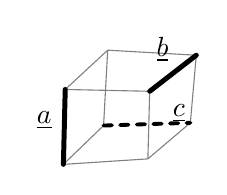
\begin{tikzpicture}[scale=.58,line cap=round]
\draw[thin,gray] (0,0)--(1.85,.12)--(2.78,.91)--(2.91,2.39)--(.97,2.50)--(.04,1.64)--(1.89,1.60)--(1.85,.12) (0,0)--(.88,.85)--(.97,2.50) (1.89,1.60)--(2.91,2.39);
\draw[line width=1.8pt] (0,0)--(.04,1.64) (1.89,1.60)--(2.91,2.39);
\draw[dashed,line width=1.4pt] (.88,.85)--(2.78,.91);
\node at (-.42,.96) {$\underline a$};\node at (2.17,2.52) {$\underline b$};\node at (2.53,1.12) {$\underline c$};
\end{tikzpicture}}

\[
 \Sigma_{a'}+\Sigma_{AC'}=\Sigma_{b'}+\deleted{\unsure{\Sigma}}\Sigma_{BC'}
\]

chacune des six dernières relations est conséquence des cinq autres, comme on voit en sommant, qui donne $0=0$!

\[
 \begin{aligned}
 &3(\Sigma_a+\Sigma_b+\Sigma_c+\Sigma_{a'}+\Sigma_{b'}+\Sigma_{c'})
 +(\Sigma_{CA'}+\Sigma_{AC'}\mathord{\text{---}}\,\mathord{\text{---}})\\
 &=(\Sigma_a+\Sigma_b\unsure{-|+}\Sigma_c+\Sigma_{a'}\unsure{-|+}\Sigma_{b'}\unsure{-|+}\Sigma_{c'})
 +3(\Sigma_{CA'}+\Sigma_{AC'}\quad)
 \end{aligned}
\]
